\documentclass[12pt,a4paper]{article}

\usepackage{verbatim} % Para incluir comentarios que abarquen varias l�neas
\usepackage[latin1]{inputenc} % Para acentos
\usepackage[spanish]{babel} % Titulos en castellano
\usepackage{hyperref}
\usepackage[pdftex]{graphicx}

\DeclareGraphicsExtensions{.pdf,.png,.jpg}

\author{Virginia Arroyo, Juli�n Oyola y Ana Ruedin \\ \normalsize \emph{Facultad de Ciencias Exactas y Naturales, Universidad de Buenos Aires}}
\title{An�lisis y detecci�n de caracter�sticas de la varicela en im�genes de la piel}
\date{}

\begin{document}

%\oddsidemargin 0in %dice al compilador de Latex que el m�rgen izquierdo ser� de 1+0 pulgadas desde el borde izquierdo de la hoja
%\textwidth 7.75in %define el ancho del texto y con esto tambi�n se puede calcular el m�rgen derecho asociado
%\topmargin 0 %coloca el margen superior del texto a 1+0 pulgadas desde el inicio de la hoja.
%\headheight 0in %define el largo del texto excluyendo el encabezado y el pie de p�gina.
%\textheight 8.5in %largo del texto

\maketitle



\begin{abstract}

\small

\emph{Las t�cnicas de procesamiento de im�genes pueden resultar de gran ayuda a los profesionales de la medicina en el diagn�stico temprano de enfermedades de la piel. Este trabajo se centra en el an�lisis y detecci�n de caracter�sticas propias de la varicela sobre fotograf�as digitales del paciente.
El procedimiento utilizado consiste en el an�lisis de la luminancia, el mejoramiento del contraste por medio de la ecualizaci�n del histograma, la suavizaci�n de la imagen y la detecci�n de bordes. Luego aplicamos operaciones morfol�gicas sobre los bordes hallados y la transformada de Hough para detectar c�rculos, teniendo en cuenta un grado de tolerancia, dado que las ampollas de la varicela no son c�rculos perfectos.
De esta forma se consigue, para un conjunto representativo de im�genes, un m�todo de detecci�n de ampollas de la varicela con una tasa razonable de aciertos.}

\paragraph{Palabras clave:}

Transformada de Hough circular, detecci�n de bordes, Canny, varicela, procesamiento digital de im�genes, representaci�n del color, filtro gaussiano, ecualizaci�n de histograma, operaciones morfol�gicas.


\end{abstract}

\section{Introducci�n}

Entre los temas m�s importantes en el procesamiento de im�genes digitales se encuentra el reconocimiento de patrones, debido a que est� relacionado con la identificaci�n de objetos. Este tema se ha tratado con distintos enfoques y t�cnicas, como puede apreciarse en trabajos tales como el de Flores y M�ndez ~\cite{AF01} del a�o 2009, que utiliza la segmentaci�n de im�genes y la detecci�n de bordes por Canny para encontrar los bordes de una oreja, o el trabajo de Rizon et al.\ ~\cite{CH01}, que utiliza segmentaci�n y CHT para detectar el contorno de cocos en una imagen. En visi�n artificial se han desarrollado m�todos para seguimiento trayectorias utilizando la transformada de Hough y el filtrado de Canny ~\cite{JJ01}. En cuanto al reconocimiento de objetos se ha propuesto m�todos para distinguir el ojo de una persona y poder realizar la medici�n del di�metro del iris ~\cite{BC01} utilizando Canny y CHT. Por otro lado, en im�genes satelitales se presentaron publicaciones donde se explica c�mo determinar la edad geol�gica de cr�teres en Marte utilizando como principales herramientas la detecci�n de bordes (Canny) y de c�rculos (CHT)~\cite{AF01}. Finalmente podemos mencionar un sistema biom�trico de reconocimiento del iris utilizando una c�mara convencional para la captura de im�genes propuesto en el art�culo ~\cite{TC01}, que presenta un m�todo que aplica Canny y luego CHT para luego normalizar el resultado de manera tal que el mismo puede ser comparado con otra captura. 

El objetivo principal de este trabajo consiste en desarrollar un m�todo capaz de detectar ampollas de varicela. Para obtenerlo trabajamos con t�cnicas de reconocimiento de patrones. La metodolog�a que utilizamos est� basada en la aplicaci�n de un preprocesamiento de la imagen y la detecci�n de bordes con Canny ~\cite{JC01} y de c�rculos con la transformada circular de Hough ~\cite{DH01} ~\cite{SJ01}.

En el desarrollo encontramos ciertas dificultades como, por ejemplo, las fotograf�as pueden estar a una escala tal que no es posible la detecci�n de las ampollas. Otro inconveniente es que las im�genes pueden tener una gran variaci�n de zonas de luz o saturaci�n de colores, lo que hace dif�cil la obtenci�n de resultados positivos. Por otro lado debemos tener presente que las ampollas suelen no ser de forma circular, como tambi�n puede ocurrir que sus bordes no se cierren, lo que hace que su detecci�n se torne compleja. Asimismo, el m�todo de detecci�n empleado puede arrojar tanto duplicaciones como falsos positivos. Para abordar cada una de estas complicaciones u obst�culos utilizamos diferentes t�cnicas aplicadas en el preprocesamiento de la imagen y el posprocesamiento de los resultados. Entre las conclusiones obtenidas, se encuentra la necesidad de aplicar m�todos de segmentaci�n para el reconocimiento de las �reas de la fotograf�a relativas a la piel.

\section{Desarrollo}

\subsection {Las im�genes de piel y sus caracter�sticas}

Las im�genes con las que se trabaj� son fotograf�as en bruto, sin ning�n tipo de tratamiento previo, tomadas con c�maras de mano, lo que hace que la calidad de las mismas sea muy variable. Uno de los principales problemas es la diferencia en la iluminaci�n de las im�genes, lo que causa zonas de luz y oscuridad muy marcadas.

Otro de los problemas es que en algunas fotograf�as los colores aparecen muy exagerados o no reales, probablemente debido a los filtros aplicados por las c�maras fotogr�ficas al momento de la captura. 

Un tema m�s a tener en cuenta es el ruido que tienen las im�genes como pueden ser lunares, pelos e inscripciones sobre las fotograf�as.

Adem�s, se debe considerar que la distancia del observador a las ampollas puede ser muy variable.

Las vesiculas de varicela en general son circulares, pero existen excepciones con formas irregulares y bordes poco definidos.

Por lo tanto, debimos extraer un subconjunto de im�genes homog�neo para procesar.

La base de datos de imagenes utilizadas pertenece a la Universidad de Iowa, publicadas en la p�gina http://hardinmd.lib.uiowa.edu/DERMPICTURES.HTML.


\subsection {Metodolog�a propuesta}

La metodolog�a propuesta consiste en una combinaci�n de t�cnicas de procesamiento de im�genes y de detecci�n de bordes. Puede resumirse en la aplicaci�n de las siguientes etapas:

\begin{enumerate}

	\item Preprocesamiento de la imagen
		\begin{enumerate}
			\item Selecci�n de un espacio de color �ptimo
			\item Ecualizaci�n del histograma
		\end{enumerate}
	
	\item Detecci�n de patrones
		\begin{enumerate}
			\item Detecci�n de bordes
			\item Aplicaci�n de operaciones morfol�gicas
			\item Detecci�n de c�rculos
		\end{enumerate}

	\item Selecci�n de candidatos
		\begin{enumerate}
			\item Detecci�n de m�ltiples ocurrencias
		\end{enumerate}

	\item An�lisis de histograma de color
		\begin{enumerate}
			\item Comparaci�n entre una ampolla y la piel normal
			\item Comparaci�n entre una ampolla de una enfermedad y otra
		\end{enumerate}

\end{enumerate}

\subsection{Preprocesamiento de la imagen}

Como primera medida a tomar realizamos un pre-procesamiento de la imagen, para poder centrarnos en un espacio de color o luminancia que maximice la detecci�n de patrones, y como paso posterior, ajustar el contraste.

La selecci�n de un espacio de color se convierte en un punto clave para el procesamiento posterior. La imagen est� compuesta por capas de luz y color que el ojo humano interpreta correctamente, pero s�lo algunas de estas capas son las m�s apropiadas para realizar la posterior detecci�n de patrones. En principio, evaluamos cuatro familias de modelos de color: RGB (RBG, CMYK), YCbCr (YUV, YCbCr), HSV (HSV, HSL) y CIE L*a*b.

Uno de los modelos de color m�s utilizados en la representaci�n de im�genes es el RGB, y su equivalente de s�ntesis sustractiva, el CYMK. Si bien este modelo de color resulta muy conveniente para la representaci�n en dispositivos como monitores o impresoras, se aparta de un principio de la visi�n humana: el ojo es m�s susceptible a cambios en iluminaci�n que a cambios en color. La luminancia es en general el componente m�s importante de la imagen al ser percibida por el ojo humano. Una imagen con un alto contraste en luminancia y pobre en cromatismo, puede ser percibida correctamente por un observador humano, mientras que el caso inverso genera dificultad en la detecci�n de patrones.

Los modelos YCbCr y L*a*b, en cambio, intentan separar la imagen en componentes de luminancia y color. De este modo, se puede contar con una capa de la imagen que representa a la misma en escalas de blanco y negro, y manipularla independientemente de la informaci�n de color, que puede incluso ser transmitida o almacenada con menor tasa de informaci�n, sin perjudicar la percepci�n humana. El modelo YCbCr es ampliamente utilizado en im�genes de video o fotograf�a. El modelo L*a*b es un derivado del espacio de color CIE XYZ, que es un intento de estandarizaci�n de la CIE del a�o 1931. Busca conseguir la uniformidad perceptiva: que ante determinados cambios en los valores de luminancia o color, la variaci�n en la percepci�n humana sea proporcional a esos cambios. La ventaja de estos modelos es que permiten diferenciar la luminancia que posee un pixel del color del mismo y, en particular, el modelo L*a*b es robusto ante cambios en la iluminaci�n.

El modelo HSV/HSB (hue, saturation, value o brightness), busca modelar la percepci�n de color de un artista, que piensa en un determinado tinte de color (hue), la saturaci�n o pureza del mismo (saturation) y el brillo o luz (value). La principal ventaja de este modelo es la facilidad para determinar o visualizar la componente del color, ya que se encuentra separada de la saturaci�n y del brillo, sin embargo, la luminancia no resulta tan f�cil de determinar, al estar separadas las variables `saturation' y `value'.

En consecuencia, en la etapa de preprocesamiento el an�lisis se realiz� en paralelo con los modelos YCbCr y L*a*b. De ambos se extrajo la componente de luminancia, es decir, $Y$ para el modelo YCbCr y $L$ en el caso de L*a*b.

Para poder incrementar el contraste global de las im�genes se realiza una ecualizaci�n del histograma, lo cual es especialmente �til cuando las �reas de inter�s consisten de valores cercanos. Justamente las im�genes tratadas cumplen con esta condici�n, ya que las mismas contienen zonas de poca diferencia de luz en la piel, donde se encuentran las ves�culas de la varicela, en comparaci�n con grandes diferencias de luz entre la piel y el fondo de la fotograf�a, usualmente oscuro.


\subsection{Detecci�n de patrones}

Los m�todos de segmentaci�n se pueden agrupar en diferentes esquemas de clasificaci�n. En un sentido amplio se pueden considerar tres tipos principales: esquemas de agrupamiento de puntos, m�todos basados en bordes y m�todos orientados a regiones ~\cite{CK01}~\cite{LK01}. Adem�s, se han propuesto esquemas h�bridos que resultan de combinaciones de los enfoques anteriores.
Para la segmentaci�n de las fotograf�as en zonas con ampollas y zonas sin ampollas utilizaremos m�todos basados en la detecci�n de bordes.

\subsubsection{Detecci�n de bordes}

Se puede definir en el Procesamiento Digital de Im�genes que un borde es la frontera entre un objeto y el fondo. Una vez identificado el borde, se puede localizar todo el objeto, as� como analizar su forma. La utilizaci�n de la informaci�n de borde nos simplifica en gran medida el an�lisis de las fotograf�as, ya que una vez identificados los bordes podemos estudiarlos y determinar si se trata de elementos circulares que puedan identificarse con ves�culas en la piel. Los objetivos principales de un detector de borde son dos: una baja tasa de error y una buena localizaci�n del borde. El primer objetivo se refiere a la capacidad del detector para clasificar pixeles de la imagen como bordes, sin incluir elementos espurios como ruidos o manchas. El segundo objetivo tiene que ver con que la propia forma del filtro puede dar lugar a una detecci�n de borde ligeramente trasladada, o incluso duplicada ~\cite{GW01}.

Para la detecci�n de bordes en las fotograf�as utilizamos el m�todo de Canny ya que es uno de los m�todos m�s importantes para realizar una detecci�n global de bordes sobre una imagen ~\cite{JC01} y es considerado uno de los m�s robustos contra el ruido (filtro �ptimo), en comparaci�n con los m�todos de Roberts, Sobel o Prewitt ~\cite{GW01}. Esta t�cnica, que se caracteriza por estar optimizada para la detecci�n de bordes diferenciales, consta de tres etapas principales: filtrado, decisi�n inicial, e hist�resis. 
La primera etapa consiste en un filtrado de convoluci�n de la derivada primera de una funci�n gaussiana normalizada discreta sobre la imagen, realizada en dos direcciones: horizontal y vertical. El objetivo de aplicar un filtro gaussiano en esta etapa es eliminar ruido de la imagen, ya que el mismo puede llevar a detectar bordes err�neamente. La funci�n gaussiana posee dos par�metros fundamentales, valor medio m, y desviaci�n t�pica sigma. En este caso, el valor medio es nulo. Por otro lado, durante las pruebas result� adecuado aplicar el filtro gaussiano con un sigma igual a 2. El paso siguiente consiste en obtener el gradiente en las direcciones vertical y horizontal y con ellos detectar picos que indiquen la presencia de un borde. La �ltima etapa de procesamiento realiza una optimizaci�n de la decisi�n llevada a cabo en la etapa anterior, mediante la aplicaci�n de una funci�n de hist�resis sobre la imagen. Esta funci�n se basa en la definici�n de dos umbrales, TL y TH, tales que TL $<$ TH. Valores t�picos para estos umbrales son 0.1 y 0.5, respectivamente, aunque se recomienda que TH y TL tengan una relaci�n entre 2:1 y 3:1, dependiendo de la relaci�n se�al ruido, en el caso de que este valor sea conocido ~\cite{JC01}. En esta etapa se realizan los siguientes c�lculos:

\begin{enumerate}

	\item Un pixel de la imagen $e$, $e(i,j$), se considera borde definitivo si $e(i,j) \geq TH$.
	\item Un pixel de la imagen $e$, $e(i,j)$, se considera fondo definitivo si $e(i,j) < TL$.
	\item Todos los pixeles en un vecindario 3 x 3 de los pixeles considerados como borde definitivo, $e(k,l)$, se consideran tambi�n borde definitivo si $e(k,l) \geq TL$.

\end{enumerate}

Durante las pruebas realizadas surgi� como �ptimo los umbrales [TL TH] iguales a [0.15 0.4], lo que implica que requiere un pixel inicial con un valor alto relativo ($\geq 0.4$) para comenzar el borde, y un pixel vecino no muy alto para continuarlo ($\geq 0.15$).

\subsubsection{Operaciones morfol�gicas}

Luego de realizar la detecci�n de bordes se recomienda realizar operaciones morfol�gicas para el cierre de contornos abiertos. Las operaciones morfol�gicas son una herramienta muy utilizada en el procesamiento de im�genes. Pueden simplificar los datos de una imagen, preservar las caracter�sticas esenciales y eliminar aspectos irrelevantes. Una de las sugerencias fue realizar una operaci�n de cierre seguida de una operaci�n de apertura.

La operaci�n de apertura suaviza el contorno de un objeto, separando peque�os enlaces entre formas presentes en la imagen. Si se toma como referencia un contorno, la apertura suaviza la imagen por la parte interior del mismo, lo cual es consecuencia de la erosi�n previa a la dilataci�n que lo caracteriza. La aplicaci�n de la apertura realiza una separaci�n de formas en una imagen. 

La operaci�n de cierre como la operaci�n de apertura, suaviza el contorno del objeto, pero por la parte exterior del mismo. Al realizarse previamente la dilataci�n, se fortalecen los enlaces d�biles entre los objetos.

Sin embargo, en nuestro caso no sirvi� realizar una operaci�n de cierre y luego una de apertura ya que esto hac�a que perdi�ramos los contornos detectados.

Otras de las operaciones morfol�gicas con las probamos fue la operaci�n `clean', que b�sicamente elimina los pixeles aislados. Esta operaci�n no mejor� resultados.

Finalmente, probamos con la operaci�n `bridge', que une pixeles que se hallan separados por un pixel. Con esta operaci�n obtuvimos mejores resultados.

\subsubsection{Detecci�n de c�rculos}

Una vez obtenidos los bordes de la imagen y eliminado todo elemento que pueda entorpecer la b�squeda de las ves�culas de la varicela, se utiliza la transformada circular de Hough para detectar dichas ves�culas.

La transformada de Hough se trata de un m�todo utilizado para detectar l�neas de alguna clase determinada, presentes en una imagen digital. En general, su aplicaci�n implica el uso de una formulaci�n de par�metros espec�fica al tipo de l�nea que se desea detectar (usualmente rectas, c�rculos o elipses). Sin embargo, puede generalizarse para cualquier tipo de forma ~\cite{AN01}.

La forma cl�sica de la transformada fue originalmente propuesta por Paul Hough en 1959 durante la conferencia internacional sobre aceleradores de alta energ�a del CERN ~\cite{HO01}. Al utilizarla para detectar l�neas rectas en una imagen, la transformada puede basarse en los dos par�metros impl�citos en la ecuaci�n de la recta seg�n la representaci�n pendiente-ordenada en el origen, $y = ax + b$.
Independientemente de la formulaci�n de par�metros empleada, la transformada siempre utiliza lo que se conoce como Arreglo de Acumulaci�n, donde se totalizan los ``votos'' que dan el resultado de los par�metros m�s apropiados al tipo de l�nea que se desea detectar.

La Transformada de Hough plantea entonces que en el espacio originado por los par�metros a y b (o espacio de Hough), es donde se analiza la aparici�n o no de una l�nea de puntos. Sin embargo, esta formulaci�n tiene algunos inconvenientes num�ricos: para rectas horizontales, cuando $a = 0$ y con rectas verticales, cuando $a\to\infty$ . Para evitar estos inconvenientes se puede reformular la transformada en la representaci�n de coordenadas polares o radio-�ngulo. Esta versi�n fue presentada por Richard Duda y Peter Hart en 1972 ~\cite{DH01}. La ecuaci�n de la recta utilizada en esta versi�n es $p = x \cos \alpha + y \sin \alpha$.

Las definiciones b�sicas de la transformada de Hough son:

\begin{enumerate}

	\item {\bf Funci�n de Par�metros de la Transformada:} Es como se describe el objeto a detectar: rectas, c�rculos, elipses.
	\item {\bf Transformada Directa de Hough:} Cada punto en el espacio de dos dimensiones de la imagen, es transformado a un hiper-espacio de Hough de n dimensiones, donde n es la cantidad de par�metros utilizados.
	\item {\bf Transformada Inversa de Hough:} Cada punto en el espacio de Hough describe una instancia espec�fica del tipo de l�nea de inter�s en el espacio bidimensional de la imagen.

\end{enumerate}

La transformada circular utiliza la siguiente f�rmula $r=(x-x_0)^2 + (y-y_0)^2$. Los par�metros de la funci�n de la transformada son: el centro del c�rculo y el radio. Es decir que el espacio de Hough es tridimensional, luego el arreglo de acumulaci�n ser� de dimensi�n tres. Esta �ltima es la versi�n que utilizamos para la detecci�n de las ves�culas de la varicela.

Una vez obtenido el Arreglo de Acumulaci�n se debe decidir con alg�n criterio si se esta en presencia de un c�rculo. En este trabajo el criterio que tomamos fue calcular un valor para cada posible c�rculo a trav�s de una ponderaci�n relativa respecto del c�rculo que obtuvo m�s votos. Luego comparamos este valor con un porcentaje de aciertos esperados. Durante las pruebas trabajamos con varios valores de este porcentaje, obteniendo resultados m�s representativos con un porcentaje del 90 por ciento. 

\subsection{Selecci�n de candidatos}

Cuando se ingresa m�s de un radio posible para la detecci�n de c�rculos, puede ocurrir que para una ves�cula haya m�s de caso positivo. Si se presenta esta circunstancia, realizamos una selecci�n sobre los c�rculos detectados en el espacio de Hough.

Consideramos que una detecci�n est� duplicada, cuando existen dos c�rculos cuyos centros distan uno del otro en menos de un cierto valor $k$. Entonces, dos c�rculos son \emph{redundantes} si cumplen que $d \leq k$, donde $d$ es la norma de la diferencia entre los centros de los c�rculos. Ante la detecci�n de estos c�rculos redundantes, seleccionamos aqu�l que tenga m�s votos en el arreglo de acumulaci�n.
En una primera aproximaci�n, trabajamos con $k = max(r1, r2)$ donde $r1$ y $r2$ son los radios, lo que equivale a que el centro del c�rculo menor se encuentra dentro del c�rculo mayor. Sin embargo, el valor de $k$ que arroj� mejores resultados emp�ricamente fue $k = r1 + r2$, lo que equivale a considerar que dos c�rculos son redundantes si sus circunferencias se intersecan. En las figura \ref{fig:deteccionDuplicadosK1K2} se puede observar la diferencia entre la detecci�n de duplicados con $k = max(r1, r2)$ y $k = r1 + r2$.

\begin{figure}
\caption{Detecci�n de c�rculos redundantes con $k = max(r1, r2)$ y $k = r1 + r2$}
\label{fig:deteccionDuplicadosK1K2}
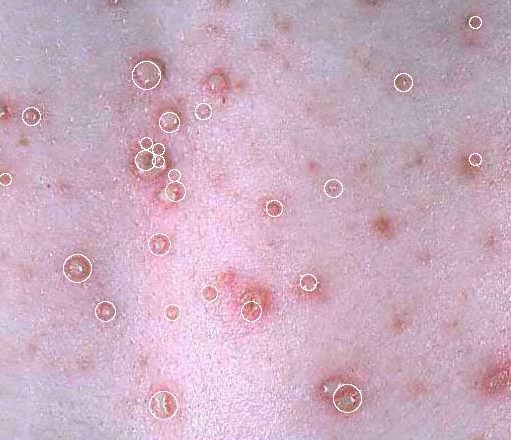
\includegraphics[scale=0.50]{Resources/resultado-chicken_pox_picture_13-int689101114.jpg}
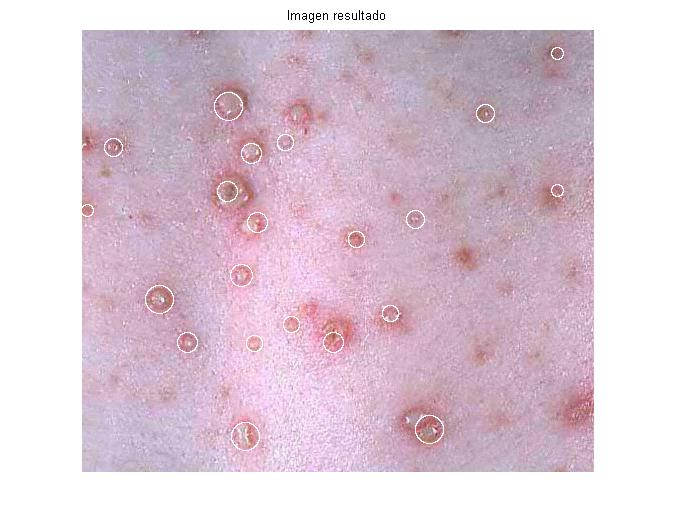
\includegraphics[scale=0.50]{Resources/resultado-chicken_pox_picture_13-int689101114-conc2.jpg}
\end{figure}



\subsection{An�lisis de histograma de color}

Una vez realizada la detecci�n de ampollas, hay dos problemas a considerar. El primero es encontrar formas de determinar si estamos en presencia de un falso positivo, el segundo es analizar si existen diferencias entre las ampollas de la varicela y las de otra enfermedad.

As� como para la detecci�n utilizamos t�cnicas basadas en la forma, para el an�lisis posterior utilizamos t�cnicas basadas en el color interno de las ampollas detectadas.
Trabajos anteriores... (TODO: completar)


\subsubsection{Comparaci�n entre una ampolla y la piel normal}

Para analizar las diferencias entre una ampolla y una regi�n de piel normal, nos centramos en analizar el histograma de las distintas componentes de color, en forma individual, y en el histograma bivariable de a pares de componentes. Dentro de los histogramas buscamos si existen patrones de concentraci�n de valores de color que nos permitan definir el sector analizado.

Nuevamente, para analizar los histogramas, se puede realizar sobre distintos espacios de color. El espacio de color L*a*b, con el que trabajamos en la etapa de detecci�n, sigue siendo conveniente porque tiene el color concentrado en dos de sus componentes (la restante es de luminancia), las cuales pueden ser analizadas en conjunto con un histograma bivariable. Adicionalmente, el espacio de color RGB puede brindar informaci�n sobre el corrimiento al rojo de las ampollas en relaci�n a la piel normal. (TODO: agregar citas)

El proceso consiste en 3 pasos:

\begin{enumerate}

	\item {\bf Selecci�n de ampollas de referencia}
	
La varicela atraviesa distintas etapas durante su desarrollo. La primera etapa luego de la incubaci�n consiste en la aparici�n de las ves�culas t�picas de la enfermedad, que contienen l�quido en su interior, lo que les da el aspecto caracter�stico (ver \ref{fig:comparacionEtapasVaricela}). Luego de esa etapa, las ves�culas se transforman en costras (ver \ref{fig:comparacionEtapasVaricela}), momento a partir del cual las lesiones ya no son contagiosas.
Para el an�lisis nos centramos en la primera etapa, seleccionando de la base de im�genes aquellas que fueran del primer estad�o de la enfermedad.

\begin{figure}
\caption{Imagen de}
\label{fig:comparacionEtapasVaricela}
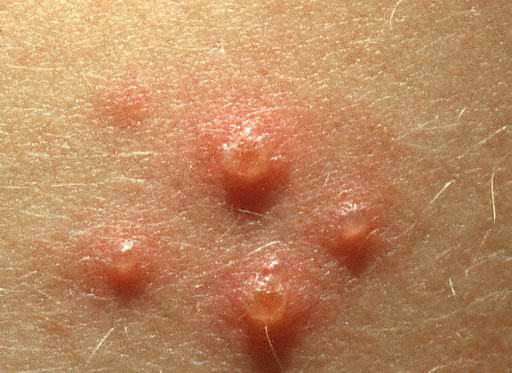
\includegraphics[scale=0.50]{Resources/chicken_pox_primary_lesions_03.jpg}
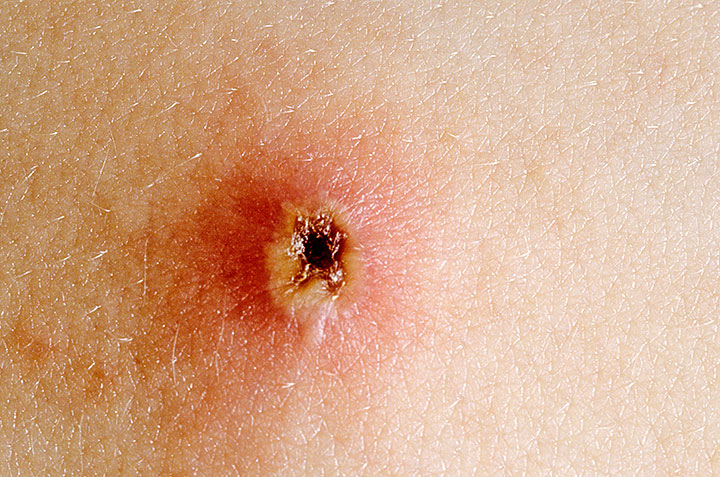
\includegraphics[scale=0.50]{Resources/varicella_18.jpg}
\end{figure}

	\item {\bf Construcci�n de un histograma promedio}
	
Para las im�genes seleccionadas, seleccionamos manualmente las ves�culas y armamos un histograma promedio con los pixels internos, para cada componente a analizar. Los histogramas son, para RGB:

		\begin{itemize}

\item Un histograma de la componente R
\item Un histograma de la componente G
\item Un histograma de la componente B
\item Un histograma bivariable de las componentes R y G
\item Un histograma bivariable de las componentes G y B
\item Un histograma bivariable de las componentes R y B

		\end{itemize}
	
	Y para LAB:

		\begin{itemize}

\item Un histograma de la componente L
\item Un histograma de la componente A
\item Un histograma de la componente B
\item Un histograma bivariable de las componentes L y A
\item Un histograma bivariable de las componentes A y B
\item Un histograma bivariable de las componentes L y B

		\end{itemize}
	
	\item {\bf An�lisis comparativo del histograma evaluado contra el promedio}
	
Dada una posible ampolla, la comparaci�n con el histograma promedio puede brindar informaci�n acerca de si estamos en presencia de un falso positivo, o tambi�n si se trata de una ampolla de la enfermedad en cuesti�n. Para poder determinarlo num�ricamente, utilizamos mediciones de distancia (o divergencia) entre histogramas. Si la distancia del histograma de la ampolla candidata al promedio est� por debajo o por encima de cierto umbral, puede ser un indicador.
	
De este modo, esperamos que:
		\begin{itemize}

			\item El histograma de la componente R presente un corrimiento hacia el rojo en el caso de las ampollas (hacia los valores m�s altos del histograma) (ver TODO: imagen histograma de ejemplo)
			\item El histograma bivariable de las componentes A y B tambi�n presente un corrimiento hacia el rojo (hacia los valores m�s altos de A y B, en la esquina superior derecha del histograma) (ver TODO: imagen histograma de ejemplo)

		\end{itemize}

			Las medidas de distancia o divergencia de histograma que utilizamos son la norma 1, la norma 2 y la divergencia de Kullback-Leibler.
			
			La norma 1 y la norma 2 ... (TODO: explicar caracter�sticas de las normas aplicadas a medici�n de distancias entre histogramas).
			
			La divergencia de Kullback-Leibler no es una distancia (no cumple con la condici�n de simetr�a), pero es un indicador de la similitud entre dos funciones de distribuci�n P y Q, en este caso los histogramas. La KLD (Kullback-Leibler Divergence) mide la cantidad esperada de bits extra requeridos para codificar ejemplos de P utilizando un c�digo basado en Q. T�picamente, P representa la distribuci�n real de datos u observaciones (en este caso, la ampolla observada), y Q representa el modelo te�rico (en este caso, el histograma promedio).
			El caso particular de la KLD que utilizamos es la sim�trica, que se obtiene como:
			KLD(P||Q) * KLD(Q||P) /2.

	Sobre los valores observados de las distancias, suponemos que se comportan como una normal, y medimos la media (acotada para eliminar el 10\% de los valores outliers) y el desv�o est�ndar. Con estos valores, inferimos una normal con la que asignamos un valor de probabilidad a nuevas ampollas. Ese valor indica cu�l es la probabilidad de que estemos en presencia de una ampolla o de un falso positivo.
			
\end{enumerate}

\subsubsection{Comparaci�n entre una ampolla de una enfermedad y otra}

Para la comparaci�n entre una ampolla de una enfermedad y otra, tomamos el mismo conjunto de im�genes evaluadas de una enfermedad y realizamos las mediciones contra el histograma promedio de esa misma enfermedad, y contra el histograma promedio de la otra, utilizando los mismos indicadores.
De este modo esperamos que:
	\begin{itemize}

			\item Las distancias o divergencias de las ves�culas de la imagen comparadas contra el histograma promedio de la enfermedad analizada, den todas dentro del rango esperado,
			\item Las distancias comparadas con el histograma de la otra enfermedad, indiquen que pocas o ninguna de las ves�culas caigan dentro del rango esperado.

	\end{itemize}


\section{Resultados}

\subsection{Resumen}

En el desarrollo encontramos ciertas dificultades. Por ejemplo, las fotograf�as pueden estar a una escala tal que no es posible la detecci�n de las ampollas, o las im�genes pueden tener una gran variaci�n de zonas de luz o saturaci�n de colores, lo que hace dif�cil la obtenci�n de resultados positivos. Por otro lado debemos tener presente que las ampollas suelen no ser de forma circular, como tambi�n puede ocurrir que sus bordes no se cierren, lo que hace que su detecci�n se torne compleja. Asimismo, el m�todo de detecci�n empleado puede arrojar tanto duplicaciones como falsos positivos. Para abordar cada una de estas complicaciones u obst�culos utilizamos diferentes t�cnicas aplicadas en el preprocesamiento de la imagen y el posprocesamiento de los resultados, y el an�lisis de las caracter�sticas de color de las ampollas en forma comparativa con la piel u otras enfermedades. Entre las conclusiones obtenidas, se encuentra la necesidad de aplicar m�todos de segmentaci�n para el reconocimiento de las �reas de la fotograf�a relativas a la piel.

\subsection{Detecci�n de las ampollas}

Para realizar la detecci�n de los ampollas, se trabaj� con los siguientes par�metros \footnote{Las funciones fueron desarrolladas en MATLAB}:
\begin{enumerate}

	\item El rango de radios esperados para las ves�culas
	\item El porcentaje de puntos del c�rculo detectado, con respecto al m�ximo de su mismo radio
	\item Distancia para detectar c�rculos redundantes
	\item Escala de la fotograf�a

\end{enumerate}

\subsubsection{El rango de radios esperados}
El algoritmo desarrollado necesita de la especificaci�n de los radios de los c�rculos a detectar.

Tomando como ejemplo la imagen de la figura \ref{fig:deteccionRadios2324} \footnote{Las im�genes utilizadas pertenecen al archivo de im�genes de la Universidad de Iowa http://www.lib.uiowa.edu/HARDIN/MD/DERMPICTURES.HTML}, se pueden realizar pruebas con diferentes radios esperados, y verificar que var�a la efectividad de la detecci�n de c�rculos. En esta prueba se puede observar claramente que la selecci�n de un radio err�neo puede determinar la aparici�n de falsos positivos, sin embargo, cuando el radio esta bien seleccionado, la detecci�n es correcta.

\begin{figure}[h]
\caption{Detecci�n con radio $r = 23$ y $r = 24$}
\label{fig:deteccionRadios2324}
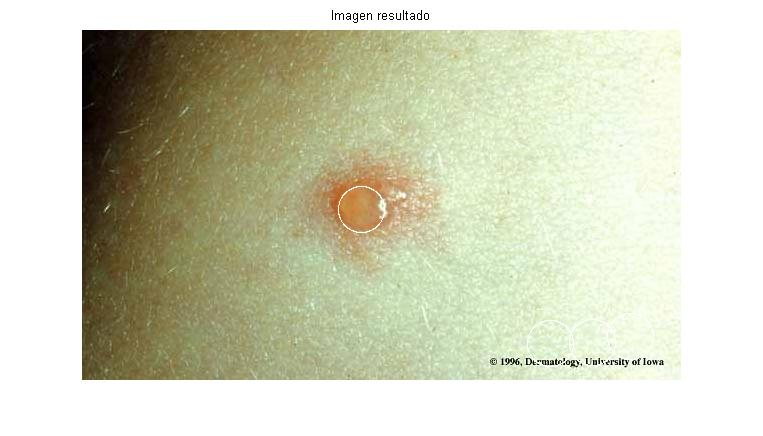
\includegraphics[scale=0.50]{Resources/resultado-Varicel-02-radio23.jpg}
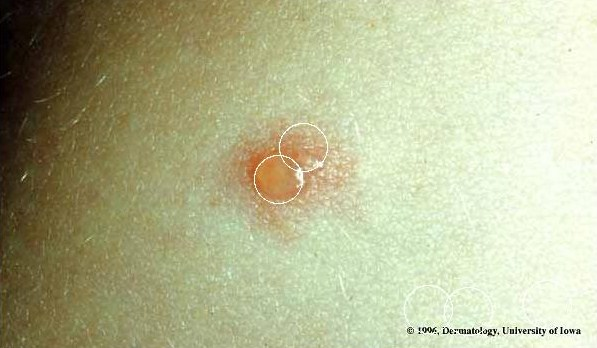
\includegraphics[scale=0.50]{Resources/resultado-Varicel-02-radio24.jpg}
\end{figure}

Sin embargo, el m�todo se muestra robusto para la imagen de la figura \ref{fig:deteccionRadios4043}, donde la ampolla es detectada con diferentes radios ingresados, a pesar de que sus bordes son claramente no circulares.

\begin{figure}[h]
\caption{Bordes y detecci�n con radio $r = 40$ y $r = 43$}
\label{fig:deteccionRadios4043}
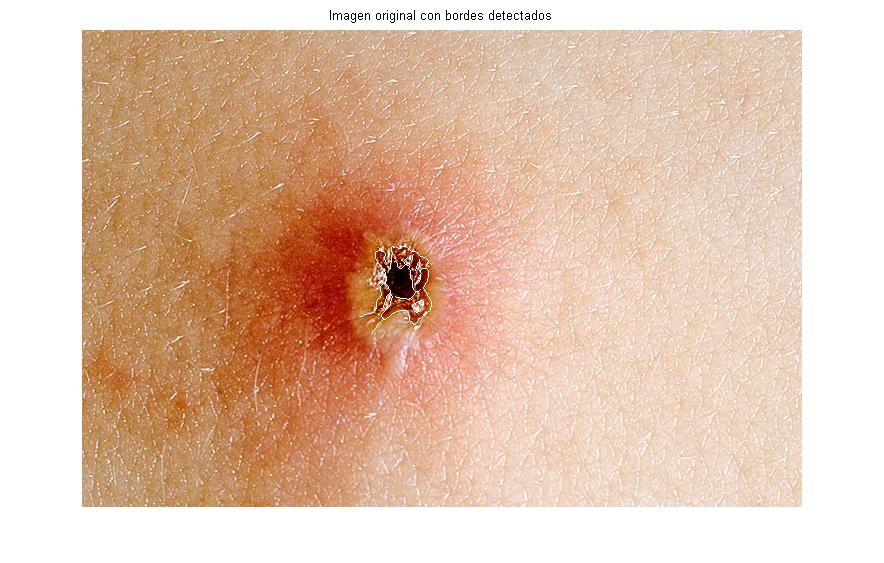
\includegraphics[scale=0.30]{Resources/resultado-varicella_18-bordes.jpg}
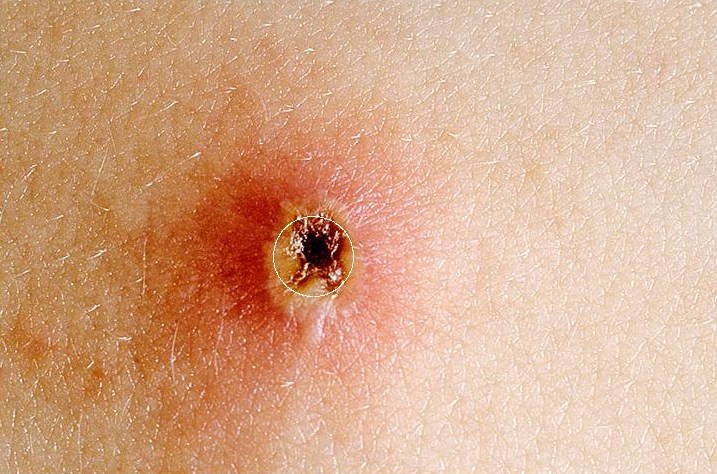
\includegraphics[scale=0.30]{Resources/resultado-varicella_18-radio40.jpg}
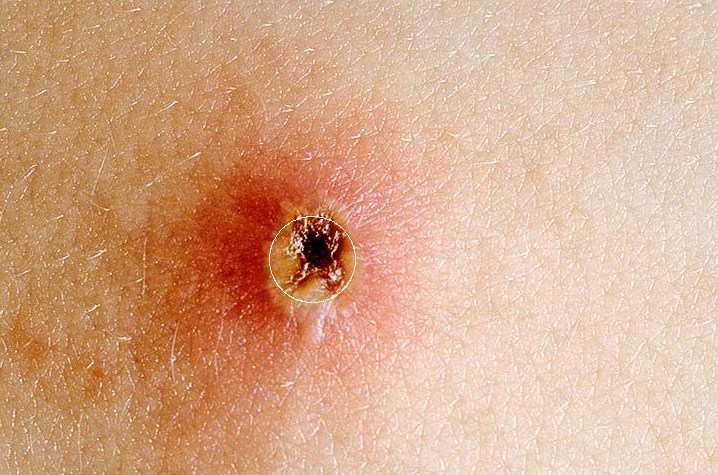
\includegraphics[scale=0.30]{Resources/resultado-varicella_18-radio43.jpg}
\end{figure}


\subsubsection{Porcentaje de puntos del c�rculo detectado}
En las pruebas realizadas, los mejores resultados fueron obtenidos con un porcentaje del 90\% de los puntos del c�rculo, ya que se minimiz� la cantidad de falsos positivos.
Tomando los resultados de evaluar la imagen de la figura \ref{fig:bordesDetectados}, se puede observar que hay dos ves�culas cuyos bordes no son circulares. Si se disminuye el umbral del porcentaje a un 70\%, son detectadas. Esto sucede porque en la fotograf�a existen otras ves�culas del mismo di�metro cuya forma es m�s cercana a un c�rculo. Por lo tanto, cuando se pondera los acumulados de una ves�cula cuya forma es m�s irregular, con los acumulados m�ximos que corresponden a ves�culas m�s circulares, sucede que las primeras no pueden detectarse ya que el porcentaje resultante es menor al 80\%.

\begin{figure}
\caption{Bordes detectados. Ampollas lejanas a la forma circular}
\label{fig:bordesDetectados}
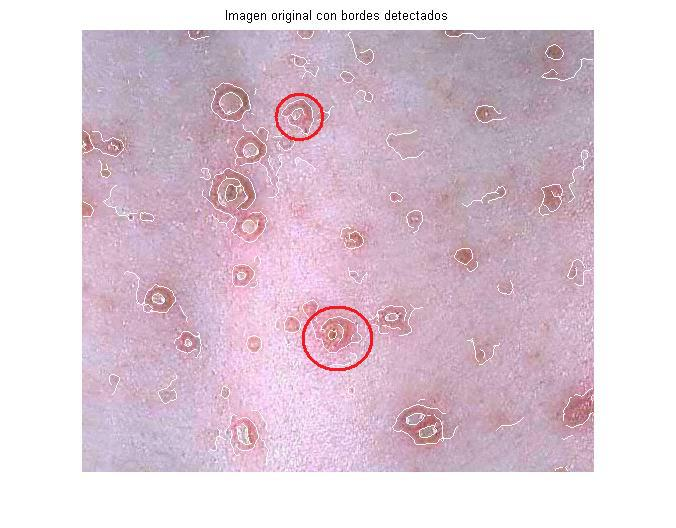
\includegraphics[scale=0.50]{Resources/resultado-chicken_pox_picture_13-marcado.jpg}
\end{figure}

\begin{figure}
\caption{Detecci�n de c�rculos con umbral = 70\% y 90\%}
\label{fig:umbralPorcentajeHough}

\includegraphics[scale=0.25]{Resources/resultado-chicken_pox_picture_13-int689101114-conc2-70.jpg}
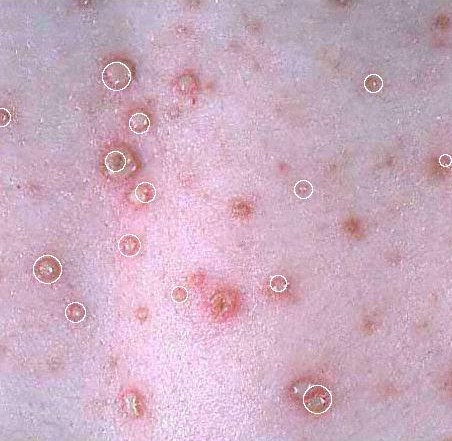
\includegraphics[scale=0.25]{Resources/resultado-chicken_pox_picture_13-int689101114-conc2-90.jpg}
\end{figure}

Para corregir este desv�o podr�amos ponderar con un porcentaje del acumulado de un c�rculo completo correspondiente al radio que estamos examinando. De esta forma la detecci�n de ves�culas irregulares no estar�a supeditada a que existan otras cuya forma son m�s cercanas al c�rculo, sino que se podr�a comparar con un porcentaje del c�rculo completo. El mismo fen�meno se puede observar en la figura \ref{fig:umbralPorcentajeHough90}.

\begin{figure}
\caption{Detecci�n de c�rculos con umbral = 90\%}
\label{fig:umbralPorcentajeHough90}
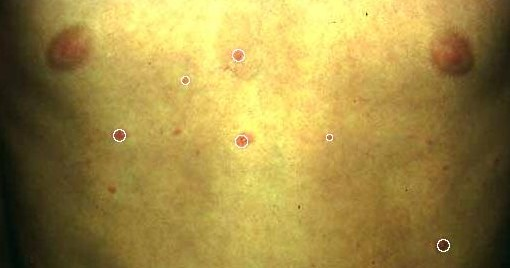
\includegraphics[scale=0.50]{Resources/resultado-Varicel-01-90.jpg}
\end{figure}


\subsubsection{Distancia para detectar c�rculos redundantes}
Inicialmente, en las pruebas para descartar detecciones duplicadas de ampollas, determinamos que dos c�rculos son redundantes cuando sus centros se encuentran a una distancia menor que el radio m�ximo. Es decir, que consideramos que dos c�rculos establecen la presencia de la misma ampolla cuando el centro del c�rculo menor, se encuentra dentro del c�rculo mayor. Sin embargo, en las pruebas realizadas con la imagen que se muestra en la figura \ref{fig:deteccionDuplicadosK1K2}, para poder descartar detecciones duplicadas se debi� modificar la distancia considerada ($k = r1 + r2$). Es decir, que si se tocan en un punto son considerados redundantes. Al realizar este cambio, el resto de las pruebas no se vieron modificadas.

\subsubsection{Escala de la fotograf�a}
Uno de los requisitos para que el m�todo presentado trabaje de manera exitosa, es que la imagen se encuentre en una escala razonable para la detecci�n de bordes y c�rculos. Por ejemplo, en la prueba con las im�genes de la figura \ref{fig:imagenesEscalaInutilizable}, se observa que, dada la escala que tienen, las ampollas no son localizadas.

\begin{figure}
\caption{Ejemplos de im�genes a escalas no utilizables}
\label{fig:imagenesEscalaInutilizable}
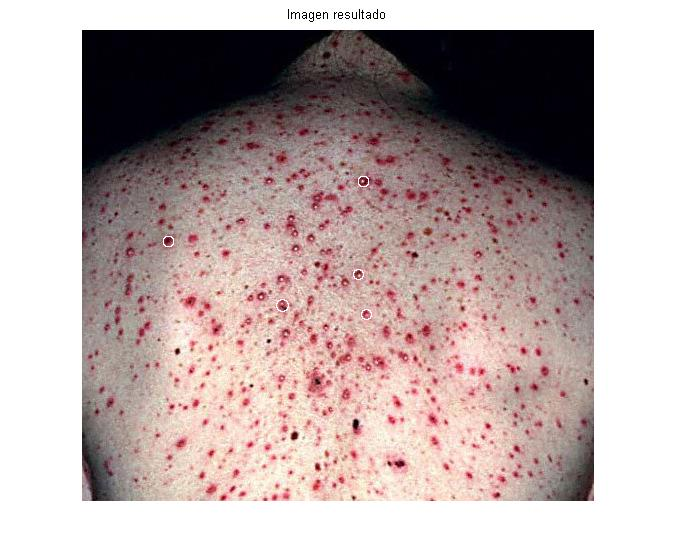
\includegraphics[scale=0.50]{Resources/resultado-chicken_pox_picture_01.jpg}
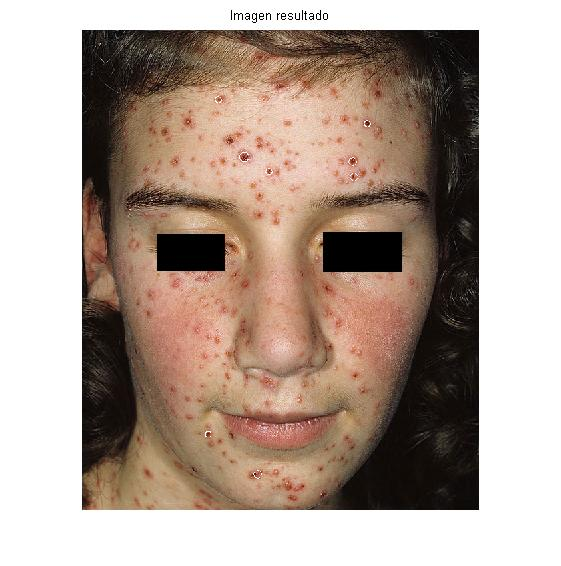
\includegraphics[scale=0.50]{Resources/resultado-varicella_9.jpg}
\end{figure}

En general se observ� un buen desempe�o del proceso para las im�genes de las figuras \ref{fig:deteccionRadios4043} y \ref{fig:imagenOk2}.


\begin{figure}
\caption{Ejemplo de detecci�n con ampollas de tama�o mediano}
\label{fig:imagenOk2}
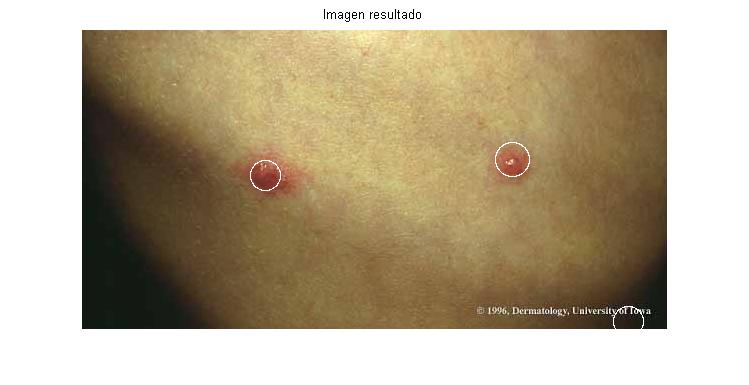
\includegraphics[scale=0.5]{Resources/resultado-Varicel-03.jpg}
\end{figure}

\begin{figure}
\caption{Ejemplo de detecci�n con ampollas de tama�o mediano}
\label{fig:imagenOk3}
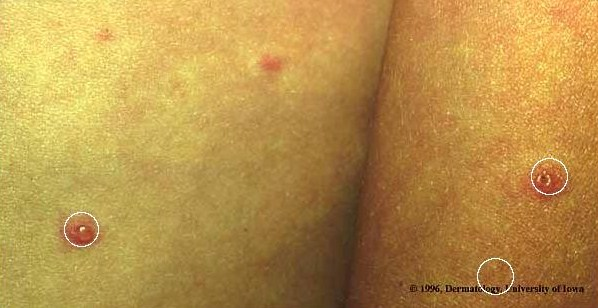
\includegraphics[scale=0.5]{Resources/resultado-Varicel-04.jpg}
\end{figure}



\subsection{An�lisis de histograma de color}

En un principio trabajamos con imagenes de varicela y herpes, tomando todas los estadios de ambas enfermedades, descartando s�lo aquellas cuya escala no permitia detectar las ampollas. Calculamos el histograma promedio y al realizar las mediciones: KLD y norma 1 y 2, no obtuvimos buenos resultados. 
Para tratar de determinar cu�l era el motivo de estos resultados, comenzamos con un analisis m�s detallado de cada uno de los histogramas de las ampollas, tanto de varicela como de herpes, y los comparamos con los histogramas de zonas de piel, respetando el tama�o de la zona de piel estudiada. Tratamos de encontrar si podiamos determinar rangos en las componentes de color A y B, a los cuales pertenecian las ampollas de varicela y herpes respectivamente. Comparamos la ampollas de varicela con zonas de piel por un lado y ampollas de herpes con zonas de piel, por otro lado. Lo que observamos fue que los rangos de las componentes A y B de las ampollas, tanto en la varicela como en el herpes, se solapaban con los rangos de dichas componentes de las zonas de piel. 

(se podria poner un grafico de los histogramas calculados mostrando el solapamiento del que hablamos)

Podemos ver que una ampolla de varicela en su primer estadio, es una ampolla con agua, que se transforma en una ampolla con c�scara, en su estadio final. Estas diferencias, entre otras cosas, muestran colores distintos, que se traducen en rangos distintos de A y B; y que por consiguiente, afectan al histograma de la ampolla y a las mediciones que hagamos sobre �l. Algo similar podemos ver en las ampollas de herpes.

Entonces nos centramos en un estadio de la enfermedad, tanto de la varicela como del herpes, para quedarnos s�lo con las caracteristicas de las ampollas de ese estadio. Calculamos nuevamente los histogramas de las ampollas, el histograma promedio y las mediciones de KLD y las normas. 
Con esta nueva muestra conseguimos mejores resultados y encontramos rangos donde podemos decir que un circulo pertenece a una ampolla o no. Este resultado lo obtuvimos tanto para varicela como para herpes. 

Adem�s, observamos que los histogramas de LAB se encuentran m�s concetrados que los histogramas de RGB, donde se ven m�s dispersos. 

(podemos poner una imagen de los histogramas)

Luego comparamos ambas enfermedades. Tomamos el histograma promedio de una de las enfermedades y las imagenes de la otra enfermedad. Por ejemplo, el histograma promedio de la varicela y las imagenes de herpes, y al rev�s.  

(Insertar tablas:
Mediciones-HerpesConHistogramaVaricela.xlsx
Mediciones-VaricelaConHistogramaHerpes.xlsx
)

En los resultados se puede observar:

\begin{itemize}

\item No hay una separaci�n clara entre los rangos de valores de KLD, norma 1 y norma 2, entre las enfermedades de varicela y herpes. Por ejemplo, para las im�genes analizadas, el rango de KLD medido entre cada histograma y el promedio, oscila entre 4,99 y 12,47 para herpes y oscila entre 6,66 y 14,47 para varicela.

\item Sin embargo, para una imagen dada, la cantidad de resultados que caen dentro de uno u otro rango permiten inclinar la balanza para decidir si la fotograf�a pertenece a una u otra enfermedad. Por ejemplo, la imagen "herpes-zoster-309", comparada utilizando KLD sobre las componentes A y B con el histograma promedio de varicela, arroja 2 valores dentro del rango y 4 por fuera, y comparada con el histograma promedio de herpes, arroja 6 resultados dentro del rango.

\item Los mejores resultados se obtuvieron comparando el histograma bivariable sobre las componentes A y B, y utilizando la divergencia KLD.

\end{itemize}


Mencionar:
- Al principio, las mediciones no dieron buenos resultados y tuvimos que centrarnos en analizar las ampollas una a una y extraer patrones
- Calculamos histogramas de cada una de las ampollas, y tratamos de determinar si ten�amos distintos rangos en las componentes de A y B, entre varicela y herpes. Nos dimos cuenta de que se solapaban, y que no bastaba una simple comparaci�n por rango para determinar.
- Nos centramos en un estad�o de la enfermedad (tanto para herpes como para varicela), y volvimos a calcular el histograma promedio.
- Apuntamos a dos objetivos: comparar ampollas con piel, y ampollas de una enfermedad con otra.
- En LAB, los histogramas est�n m�s concentrados, en RGB los valores est�n m�s dispersos.
- Al volver a calcular con estas directrices, encontramos diferencias entre piel y no piel.
- Finalmente, comparamos herpes con varicela.


La posibilidad de eliminar los falsos positivos aplicando t�cnicas de comparaci�n del color dentro y fuera del c�rculo, para determinar si las variaciones de color y luminancia corresponden a una ampolla de varicela.



\section{Discusi�n}

La metodolog�a presentada permite la detecci�n eficaz de ampollas de la varicela, bajo las condiciones de escala descriptas. El m�todo propuesto consiste en la aplicaci�n de diferentes t�cnicas de procesamiento de im�genes, entre ellas, Canny y CHT. Se comprobaron emp�ricamente los resultados esperados utilizando fotograf�as en bruto, demostrando un excelente desempe�o.

Para poder contar con un m�todo m�s robusto se deben abordar ciertos aspectos no tratados en este trabajo. Uno de ellos consiste en poder realizar una detecci�n de las �reas de la piel, por medio de alg�n m�todo de segmentaci�n por color. Esto permitir�a poder trabajar sobre las �reas de inter�s de la fotograf�a. Existen numerosos antecedentes de trabajos de detecci�n de piel por segmentaci�n que pueden aplicarse para mejorar los resultados obtenidos hasta el momento (ver ~\cite{RA01}, ~\cite{LC01} y ~\cite{DM01}). La mayor�a de ellos trabajan sobre modelos de color como YCbCr y HSI para reconocer secciones de piel, utilizando t�cnicas de ecualizaci�n del histograma, extrapolaci�n de pixeles y filtros de suavizaci�n.

Otro aspecto a mejorar es la detecci�n de c�rculos cuando las ampollas no tienen una forma circular, por ejemplo, considerando elipses en lugar de c�rculos. Tambi�n se puede optimizar la evaluaci�n del arreglo de acumulaci�n de CHT para que pondere los votos de cada posible c�rculo contra un porcentaje de un c�rculo completo correspondiente al radio examinado, en lugar de comparar contra el m�ximo local. Asimismo, otra variante para esta evaluaci�n consiste en considerar la direcci�n del gradiente de un punto a la hora de sumar votos en la detecci�n de c�rculos (ver Rojas, Sanz, Arteaga ~\cite{TR01}).

Un aspecto adicional a considerar es la posibilidad de eliminar los falsos positivos aplicando t�cnicas de comparaci�n del color dentro y fuera del c�rculo, para determinar si las variaciones de color y luminancia corresponden a una ampolla de varicela.

% Aplicar otros algoritmos que vimos de cierre de bordes?

\noindent{\textbf{Agradecimientos}}

Queremos dar las gracias a nuestras familias y amigos por el apoyo incondicional.

\begin{thebibliography}{200}

\small

\bibitem{RA01} Ramello, Pedro Mart�n.
``Comparaci�n de m�todos de detecci�n de piel en modelos de color YCbCr y HSI para reconocimiento de caras'', 2005.

\bibitem{LC01} Luis Coll, Dante Chinchilla, Constanza Coll, Fernando Stengel, Horacio Cabo.
``An�lisis digital de im�genes en lesiones pigmentadas de la piel. Diagn�stico precoz del melanoma'', 2007.

\bibitem{JA01} Jes�s Angulo, Jean Serra.
``Segmentaci�n de im�genes en color utilizando histogramas bi-variables en espacios color polares luminancia/saturaci�n/matiz'',
\emph{Revista ``Computaci�n y Sistemas''}, Vol.\ 8, No.\ 4, June 2005.

\bibitem{CH01} Mohamed Rizon, Haniza Yazid, Puteh Saad, Ali Yeon Md Shakaff, Abdul Rahman Saad, Masanori Sugisaka, Sazali Yaacob, M.Rozailan Mamat, M.Karthigayan.
``Object Detection using Circular Hough Transform'',
\emph{American Journal of Applied Sciences 2 (12)}: 1606-1609, 2005, ISSN 1546-9239, \copyright 2005 Science Publications.

\bibitem{SJ01} Simon Just Kjeldgaard Pedersen.
``Circular Hough Transform'',
\emph{Aalborg University, Vision, Graphics, and Interactive Systems}, November 2007.

\bibitem{MF01} Marlon Fabi�n Mac�as S�nchez, Patricia X. Ch�vez Burbano.
``Detecci�n de rostros humanos en posici�n frontal en im�genes a color utilizando propiedades estad�sticas de la piel humana junto con el m�todo de concordancia con el rostro plantilla'',
\emph{Revista Tecnol�gica ESPOL}, 2010,
http://www.dspace.espol.edu.ec/handle/123456789/9113.

\bibitem{AF01} Alejandro Flores-M�ndez, Ana Ant�gona M�ndez-Cuanalo.
``Detecci�n estable de los bordes de la oreja en im�genes 2D'',
\emph{Computaci�n y Sistemas, Vol. 13}, 2009.

\bibitem{AF02} Alejandro Flores M�ndez
``Reconocimiento y clasificaci�n de cr�teres a partir de im�genes satelitales''.
Disponible en: http://www.ci.ulsa.mx/~aflores/mars/mars-complete.html

\bibitem{DD01} David Delgado G�mez, Jens Michael Carstensen, Bjarne Ersboll, Lone Skov, Bo Bang.
``Building an image-based system to automatically score psoriasis''

\bibitem{MM02} Mariana del Fresno, Mario Moreno, Marcelo V�nere.
``Segmentaci�n de regiones de inter�s en im�genes m�dicas'',
\emph{VIII Simposio Argentino de Inform�tica y Salud}, 2005

\bibitem{MJ01} Michael J. Jones, James M. Rehg.
``Statistical Color Models with Application to Skin Detection'',
\emph{International Journal of Computer Vision }, 1999

\bibitem{DM01} Dar�o de Miguel Benito.
``Detecci�n autom�tica del color de la piel en im�genes bidimensionales basado en el an�lisis de regiones'', 2005

\bibitem{CK01} K. Castleman.
``Digital Image Processing'', Prentice Hall, 1996

\bibitem{LK01} Lakare S., Kaufman A.
``3D Segmentation techniques for medical volumes'', 
\emph{Center for Visual Computing, Department of Computer Science, State University of New York, Research Proficiency Exam}, Dic. 2000

\bibitem{GW01} R.C. Gonz�lez, R.E. Woods.
``Digital Image Processing'', Addison-Wesley, 1993.

\bibitem{JC01} J.F. Canny.
``A Computational Approach to Edge Detection'', 
\emph{IEEE PAMI}, 8(6), 1986, pp. 679-698.

\bibitem{AN01} A. Aguado y M. Nixon.
``A new Hough Transform mapping for ellipse detection''
\emph{University of Southampton Research Journal}, 1995 
http://www.ecs.soton.ac.uk/publications/

\bibitem{DH01} Richard O. Duda y Peter E. Hart.
``Use of the Hough trasformtion to detect lines and curves in pictures'', April 1971

\bibitem{TR01} Teddy Rojas, Wilmer Sanz y Francisco Arteaga.
``Sistema de Visi�n por Computadora para la Detecci�n de Objetos Esf�ricos a trav�s de la Transformada Circular de Hough''

\bibitem{BC01} Arturo Bianchetti y Silvia Ana Comastri.
``Desarrollo de una metodolog�a para medir el di�metro pupilar ocular a partir del procesado de im�genes conteniendo el ojo'', Noviembre 2008.
Documento de Trabajo N� 221, Universidad de Belgrano.
Disponible en la red: http://www.ub.edu.ar/investigaciones/dt\_nuevos/221\_bianchetti.pdf

\bibitem{JJ01} Juan Catuche, Julio Sterling, Bladimir Bacca-Cortes.
``Seguimiento de trayectorias y objetivos en tierra usando un dirigible y visi�n artificial'', Diciembre 2009.
\emph{Grupo de Investigaci�n en Percepci�n y Sistemas Inteligentes, Universidad del Valle, Escuela de Ingenier�a El�ctrica y electr�nica, Cra. 91 No. 28-23, Cali, Valle, Colombia}

\bibitem{TC01} Lucas D. Terissi, Lucas Cipollone y Patricio Baldino.
``Sistema de Reconocimiento de Iris'', 2000.
\emph{Laboratorio de Sistemas Din�micos y Procesamiento de la Informaci�n FCEIA, Universidad Nacional de Rosario Riobamba 245 bis, Rosario, Argentina}

\bibitem{HO01} Hough, P. V. 
``Machine analysis of bubble chamber pictures. In International Conference on High Energy Accelerators and Instrumentation'', 1959
\emph{(L. Kowarski, ed.) 554--556. CERN.}

\end{thebibliography}

\paragraph{Datos de Contacto}

\emph{
\\Virginia In�s Arroyo
\\Universidad de Buenos Aires, Facultad de Ciencias Exactas y Naturales, Departamento de Computaci�n.
\\Pabell�n I, Ciudad Universitaria (C1428EGA), Buenos Aires, Argentina.
\\virginia.arroyo@gmail.com
}

\emph{
\\Juli�n Ricardo Oyola
\\Universidad de Buenos Aires, Facultad de Ciencias Exactas y Naturales, Departamento de Computaci�n.
\\Pabell�n I, Ciudad Universitaria (C1428EGA), Buenos Aires, Argentina.
\\joyola@dc.uba.ar
}


\end{document}
